\documentclass[chi_draft]{sigchi}

% Use this section to set the ACM copyright statement (e.g. for
% preprints).  Consult the conference website for the camera-ready
% copyright statement.

% Copyright
\CopyrightYear{2017}
%\setcopyright{acmcopyright}
\setcopyright{acmlicensed}
%\setcopyright{rightsretained}
%\setcopyright{usgov}
%\setcopyright{usgovmixed}
%\setcopyright{cagov}
%\setcopyright{cagovmixed}
% DOI
\doi{} %http://dx.doi.org/10.475/123_4}
% ISBN
\isbn{} %123-4567-24-567/08/06}
%Conference
\conferenceinfo{IoT'17,}{October 22--25, 2017, Linz, Austria}
%Price
\acmPrice{\$15.00}

% Use this command to override the default ACM copyright statement
% (e.g. for preprints).  Consult the conference website for the
% camera-ready copyright statement.

%% HOW TO OVERRIDE THE DEFAULT COPYRIGHT STRIP --
%% Please note you need to make sure the copy for your specific
%% license is used here!
% \toappear{
% Permission to make digital or hard copies of all or part of this work
% for personal or classroom use is granted without fee provided that
% copies are not made or distributed for profit or commercial advantage
% and that copies bear this notice and the full citation on the first
% page. Copyrights for components of this work owned by others than ACM
% must be honored. Abstracting with credit is permitted. To copy
% otherwise, or republish, to post on servers or to redistribute to
% lists, requires prior specific permission and/or a fee. Request
% permissions from \href{mailto:Permissions@acm.org}{Permissions@acm.org}. \\
% \emph{CHI '16},  May 07--12, 2016, San Jose, CA, USA \\
% ACM xxx-x-xxxx-xxxx-x/xx/xx\ldots \$15.00 \\
% DOI: \url{http://dx.doi.org/xx.xxxx/xxxxxxx.xxxxxxx}
% }

% Arabic page numbers for submission.  Remove this line to eliminate
% page numbers for the camera ready copy
% \pagenumbering{arabic}

% Load basic packages
\usepackage{balance}       % to better equalize the last page
\usepackage{graphics}      % for EPS, load graphicx instead 
\usepackage[T1]{fontenc}   % for umlauts and other diaeresis
\usepackage{txfonts}
\usepackage{mathptmx}
\usepackage[pdflang={en-US},pdftex]{hyperref}
\usepackage{color}
\usepackage{booktabs}
\usepackage{textcomp}

% Some optional stuff you might like/need.
\usepackage{microtype}        % Improved Tracking and Kerning
% \usepackage[all]{hypcap}    % Fixes bug in hyperref caption linking
\usepackage{ccicons}          % Cite your images correctly!
% \usepackage[utf8]{inputenc} % for a UTF8 editor only

% Custom packages

\usepackage{paralist}
\usepackage{enumitem}

\usepackage{tikz}
\usetikzlibrary{shadows,shapes}
\usepackage{pgfplots}
\pgfplotsset{compat=1.10}

\usepackage{xcolor}
\usepackage{colortbl}
\definecolor{Gray}{gray}{0.90}

\usepackage{algorithm}
\usepackage{algorithmicx}
\usepackage{algpseudocode}

% If you want to use todo notes, marginpars etc. during creation of
% your draft document, you have to enable the "chi_draft" option for
% the document class. To do this, change the very first line to:
% "\documentclass[chi_draft]{sigchi}". You can then place todo notes
% by using the "\todo{...}"  command. Make sure to disable the draft
% option again before submitting your final document.
\usepackage[textsize=tiny, textwidth=1.3cm, disable]{todonotes}
\newcommand{\TODO}[1]{\todo[inline]{#1}}
\newcommand{\Abhishek}[1]{\todo[color=yellow!50, linecolor=black!50]{\textbf{Abhishek}: #1}}
\newcommand{\Aron}[1]{\todo[color=green!40, linecolor=black!50]{\textbf{Aron}: #1}}
\newcommand{\Doug}[1]{\todo[color=red!40, linecolor=black!50]{\textbf{Doug}: #1}}

%\usepackage[normalem]{ulem}
%\newcommand{\change}[2]{\textcolor{red}{\sout{#1}} \textcolor{blue}{#2}}
\newcommand{\change}[2]{#2} % DO NOT DISPLAY CHANGES

\newcommand{\circled}[1]{\tikz[baseline=(char.base)]{\node[shape=circle, draw, inner sep=0.5pt, solid] (char) {#1};}}
            
\newcommand{\field}[1]{\texttt{#1}}

% Paper metadata (use plain text, for PDF inclusion and later
% re-using, if desired).  Use \emtpyauthor when submitting for review
% so you remain anonymous.
\def\plaintitle{Providing Privacy, Safety, and Security in IoT-Based Transactive Energy Systems using Distributed Ledgers}
\def\plainauthor{First Author, Second Author, Third Author}
\def\emptyauthor{}
\def\plainkeywords{Internet of Things; blockchain; transactive energy; privacy; security; transactive microgrid; smart grid; anonymity.}
\def\plaingeneralterms{Design, Human Factors, Reliability, Security} % TODO: revise

% llt: Define a global style for URLs, rather that the default one
\makeatletter
\def\url@leostyle{%
  \@ifundefined{selectfont}{
    \def\UrlFont{\sf}
  }{
    \def\UrlFont{\small\bf\ttfamily}
  }}
\makeatother
\urlstyle{leo}

% To make various LaTeX processors do the right thing with page size.
\def\pprw{8.5in}
\def\pprh{11in}
\special{papersize=\pprw,\pprh}
\setlength{\paperwidth}{\pprw}
\setlength{\paperheight}{\pprh}
\setlength{\pdfpagewidth}{\pprw}
\setlength{\pdfpageheight}{\pprh}

% Make sure hyperref comes last of your loaded packages, to give it a
% fighting chance of not being over-written, since its job is to
% redefine many LaTeX commands.
\definecolor{linkColor}{RGB}{6,125,233}
\hypersetup{%
  pdftitle={\plaintitle},
% Use \plainauthor for final version.
%  pdfauthor={\plainauthor},
  pdfauthor={\emptyauthor},
  pdfkeywords={\plainkeywords},
  pdfdisplaydoctitle=true, % For Accessibility
  bookmarksnumbered,
  pdfstartview={FitH},
  colorlinks,
  citecolor=black,
  filecolor=black,
  linkcolor=black,
  urlcolor=linkColor,
  breaklinks=true,
  hypertexnames=false
}

% create a shortcut to typeset table headings
% \newcommand\tabhead[1]{\small\textbf{#1}}

% End of preamble. Here it comes the document.
\begin{document}

\allowdisplaybreaks

\title{\plaintitle}

\numberofauthors{3}
\author{%
%  \alignauthor{Leave Authors Anonymous\\
%    \affaddr{for Submission}\\
%    \affaddr{City, Country}\\
%    \email{e-mail address}}\\
%  \alignauthor{Leave Authors Anonymous\\
%    \affaddr{for Submission}\\
%    \affaddr{City, Country}\\
%    \email{e-mail address}}\\
%  \alignauthor{Leave Authors Anonymous\\
%    \affaddr{for Submission}\\
%    \affaddr{City, Country}\\
%    \email{e-mail address}}\\
}

\maketitle

\begin{abstract}
Power grids are undergoing major changes due to rapid growth in
renewable energy resources and improvements in battery technology.
While these changes enhance sustainability and efficiency, they also
create significant management challenges as the complexity of power
systems increases.  To tackle these challenges, decentralized
Internet-of-Things (IoT) solutions are emerging, which arrange local
communities into transactive microgrids.  Within a transactive
microgrid, ``prosumers'' (i.e., consumers with energy generation and
storage capabilities) can trade energy with each other, thereby
smoothing the load on the main grid using local supply.  It is hard,
however, to provide security, safety, and privacy in a decentralized
and transactive energy system.  On the one hand, prosumers' personal
information must be protected from their trade partners and the system
operator.  On the other hand, the system must be protected from
careless or malicious trading, which could destabilize the entire
grid.  This paper describes \change{our}{\emph{Privacy-preserving
    Energy Transactions} (PETra)}, which is secure and safe solution
for transactive microgrids that enables consumers to trade energy
without sacrificing their privacy.  \change{Our solution}{PETra}
builds on distributed ledgers, such as blockchains, and provides
anonymity for communication, bidding, and trading.
\end{abstract}

% TODO!
\category{K.6.m}{Miscellaneous}{Security}
\category{D.4.7}{Organization and Design}{Distributed systems}

\keywords{\plainkeywords}

%!TEX root = paper.tex
\section{Introduction}


Transactive energy models have been proposed as a set of market based mechanisms for balancing the demand and generation of energy in communities \cite{kok2016society,cox2013structured,melton2013gridwise}.
 In this approach, customers on the same feeder (i.e. sharing a power line link) can operate in an open market, trading and exchanging generated energy locally. Distribution System Operators can be the custodian of this market, while still meeting the net demand \cite{7462854}. Blockchains have  recently emerged as a foundation for enabling the transactional service in the microgrids. For example, the Brooklyn Microgrid
(\url{brooklynmicrogrid.com}) is a peer-to-peer market for locally
generated renewable energy, which was developed by LO3 Energy as a pilot project. Similarly, RWE, and Grid Singularity have developed blockchain based solutions for incentivizing neighbors to sell excess energy to the grid and payments for electric car charging %and (c) enabling pre-paid transactions for electric bills in South Africa, respectively. 
However, those solutions do not address the requirements for off-blockchain communication network and the requirements for privacy. 
 
 
 %Due to a number of challenges, however, these services have been restricted in the present to some pilot programs like Demand/Response \cite{7462854}.  On one hand, transactive energy is a decentralized power system controls problem \cite{7452738}, requiring strategic microgrid control to maintain the stability of the community and the utility. On the other hand, it is a distributed market problem where erroneous as well as malicious transactions can create a gap between demand and supply, eventually destabilizing the system.  Furthermore, this system inherently induces a distributed  infrastructure comprised of smart meters, feeders, smart inverters, utility substations, the utility central offices, and the transmission system operator, which has to provide the necessary computation fabric to support the interplay between the energy control and the fiscal market challenges.
 
 

Specifically, while blockchains provide the necessary ledger services, we still need a  communication network for sending control commands from the DSO to the prosumers as well as initiating the trade matching mechanisms.
%as described by our recent publication \textcolor{red}{\cite{Laszka17}}. 
Additionally, this communication network and the blockchain itself must preserve the privacy of the prosumers. Energy usage patterns (actual or predicted) are sensitive, personally identifiable data. Legal requirements and security considerations make it mandatory to provide a mechanism to hide the identities and transaction patterns of trade partners. Additionally, solutions must also satisfy security and safety requirements, which often conflict with privacy goals. For example, to prevent a prosumer from destabilizing the system through careless or malicious energy trading, a transactive grid must check all of the prosumer's transactions. In a decentralized system, these checks require disseminating information, which could be used to infer the prosumer's future energy consumption. 

%This paper first describes mechanisms to implement anonymity in both the communication and transactional dimensions 

In \cite{Laszka17}, we introduced {\it Privacy-preserving Energy Transactions
(PETra)}, which is our distributed-ledger based solution that
(1) enables trading energy futures in a secure and verifiable
manner, (2) preserves prosumer privacy, and (3) enables distribution system operators to regulate trading and enforce the safety rules. In this paper, we  extend the communication and transaction anonymity mechanisms. The key contributions of this paper are (a) a survey of the key concepts required for implementing the anonymity across the two dimensions, (b) a discussion on the threats that must be considered when we implement the anonymization mechanisms, and lastly (c) a discussion on implementing the anonymization extensions in PETra. 
%This paper describes privacy-aspects of the communication and transactional components of transactive microgrids. Specifically, we analyze two existing schemes for communication anonymity and two schemes for transaction anonymity. They are analyzed with respect to security and known attacks. The schemes are also judged for appropriateness in regards to their application in transactive microgrids. Based on the analysis, we propose a novel design for achieving communication and transaction anonymity in transactive microgrids.
% REDUNDANT OUTLINE
% The outline of this paper is as follows. We first summarize the transaction workflow described in \cite{Laszka17}. Thereafter, we focus on the key contributions of this paper, a discussion on the privacy challenges for both communication as well as transactions.  

% This paper introduces Privacy-preserving Energy Transactions (PETra), which is our distributed-ledger based solution that (1) enables trading energy futures in a secure and verifiable manner, (2) preserves prosumer privacy, and (3) enables DSOs to regulate trading and enforce certain safety rules. 

The outline of this paper is as follows. We first present an overview of the PETra workflow described in \cite{Laszka17} in Section \ref{sec:petra}. We then discuss the communication anonymity extensions in Section \ref{comm} and transaction anonymity in Section \ref{trans}. Section \ref{commthreat} discusses the threat vectors for the communication anonymity approach. Section \ref{transthreat} describes the transaction anonymity threats.
Finally, we provide concluding remarks in Section~\ref{sec:discussion}.

\section{Preliminaries and Requirements}

\subsection{Transactive Microgrid Components}

Here, we describe a basic system model of transactive microgrids.
We discuss the following components: a distributed ledger for recording transactions, a bid storage service that facilitates finding trade partners, a microgrid controller for regulating the microgrid load, and smart meters for measuring energy production and consumption.

\subsubsection{Distributed Ledger}
The ledger permanently stores transactions that specify energy trades, change regulatory policies for the microgrid, etc.
For providing security and safety, it is crucial that transactions are non-malleable, that is, once a transaction has been recorded, it cannot be modified or removed from the ledger.
However, for the sake of fault tolerance, the ledger also needs to be distributed.
Since a distributed ledger is maintained by multiple nodes, a key implementation requirement is reaching consensus on which transactions are valid and stored in the ledger.
Further, this consensus must be reached quickly and reliably, even in the presence of faulty or malicious (e.g., compromised) ledger nodes.
In this paper, we assume that a distributed ledger service is available, but do not make any assumption about the implementation, such as the particulars of the consensus algorithm.
In practice, a distributed ledger can be implemented using, for example, \emph{blockchains} with proof-of-stake consensus or Practical Byzantine Fault Tolerance algorithm~\cite{castro1999practical}.

\subsubsection{Bid Storage Service}
Although individual prosumers trade energy with each other, for the sake of scalability, we need a service that enables prosumers to find trade partners.
%A bid storage service receives energy buy and sell bids from prosumers, stores these 
We assume that there is a bid storage service that enables prosumers to post and read energy \emph{bids} and \emph{asks}.\footnote{A \emph{bid} is an offer to buy at a certain price, while an \emph{ask} is an offer to sell at a certain price.}  
This service relieves prosumers from communicating with a large number of potential trade partners, since they only have to communicate with the service in order to discover trade partners.
Moreover, in addition to simply storing bids and asks, the service may also find matches in the posted bids and asks, and it may notify the posting prosumers of the trade opportunity.
Note that
%Even though the bid storage appears to the nodes as one entity, 
for the sake of scalability and reliability, this service can also be implemented in a distributed manner, using multiple nodes.

\subsubsection{Microgrid Controller}
The microgrid controller is responsible for stabilizing load within the microgrid and controlling it based on the expected load in the rest of the grid.
To this end, the controller first estimates the expected load in the microgrid based on the bids and asks in the bid storage as well as on outstanding energy trades in the ledger.
By combining this estimate with the expected load in the remainder of the grid, the controller produces a control signal that specifies how much the microgrid load should be decreased or increased.
Finally, based on this control signal, the controller updates the price policy for the microgrid to influence energy production and consumption.

\subsubsection{Smart Meters}
\TODO{measures energy production / consumption}
\TODO{may record energy production / consumption on the ledger or directly report it to the DSO} 

\subsection{Requirements}

\subsubsection{Security}
Prosumers (or outside attackers) should not be able to tamper with measured energy production and consumption values, with financial balances, with other prosumers' bids.
\TODO{ensure correct billing (i.e., prosumer cannot tamper with energy production / consumption or financial balances of any prosumer)}
\TODO{ensure that prosumers cannot back out of trades unilaterally, or tamper with other prosumers trading or bids}
\TODO{ensure that prosumers cannot change policies that are to be set by the DSO for the microgird}
\TODO{impact of node compromise is limited, and can be mitigated (i.e., offending node may be removed)}

\subsubsection{Safety}
A careless or malicious prosumer may destabilize the grid by promising to produce (or consume) a large amount of energy, but failing to deliver.
\TODO{this could destabilize the microgrid, or even the main grid}
Trades which are unlikely to be delivered and would result in a gap between actual production and demand should be prevented.
\TODO{net amount of energy sold (or bought) by a prosumer is limited (by a constant set by the DSO), where net amount of energy sold is the difference between the amount of energy sold and bought (net amount of energy bought is defined analogously)}
\TODO{energy bids posted by the prosumer are limited in the same way}

\subsubsection{Privacy} 
Energy trading should not compromise the privacy of prosumers.
More specifically, prosumers' private information, including energy consumption and production values, are available only to the DSO.
\TODO{other prosumers should not be able to tell how much energy was consumed / produced by a prosumer, or what bids the prosumer has posted (or with whom the prosumer traded}




\section{Solution}

In this section, we describe our solution for providing privacy for prosumers without compromising the safety and security of the microgrid.
Figure~\ref{fig:softwareArchitecture} shows a high-level overview of the architecture of our solution.

\begin{figure}[h!]
\center
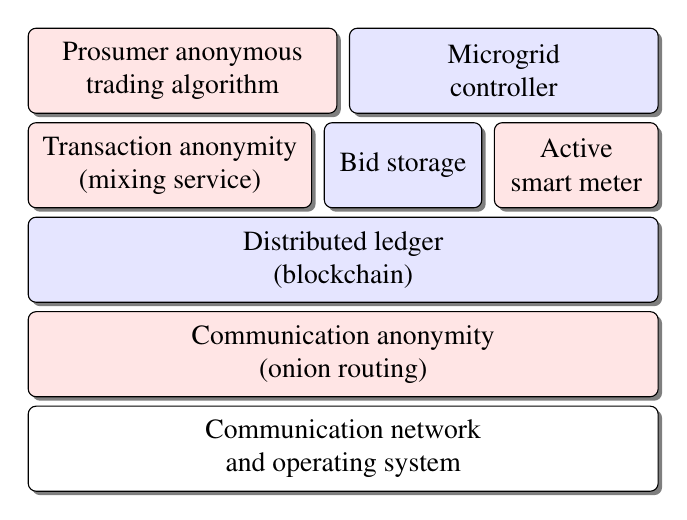
\begin{tikzpicture}[x=8cm, y=1.2cm,
  nodeStyle/.style={rounded corners=0.1cm, drop shadow={shadow xshift=0.05cm, shadow yshift=-0.05cm, fill=black}}
]
\draw [nodeStyle, fill=white]   (0, 0) rectangle    (1, 0.9) node [midway, align=center] {Communication network\\and operating system};

\draw [nodeStyle, fill=red!10]  (0, 1) rectangle    (1, 1.9) node [midway, align=center] {Communication anonymity\\(onion routing)};

\draw [nodeStyle, fill=blue!10] (0, 2) rectangle    (1, 2.9) node [midway, align=center] {Distributed ledger\\(blockchain)};

\draw [nodeStyle, fill=red!10]  (0,    3) rectangle (0.45, 3.9) node [midway, align=center] {Transaction anonymity\\(mixing service)};
\draw [nodeStyle, fill=blue!10] (0.47, 3) rectangle (0.72, 3.9) node [midway, align=center] {Bid storage};
\draw [nodeStyle, fill=red!10 ] (0.74, 3) rectangle (1,    3.9) node [midway, align=center] {Active\\smart meter};

\draw [nodeStyle, fill=red!10] (0,    4) rectangle (0.49, 4.9) node [midway, align=center] {Prosumer anonymous\\trading algorithm};
\draw [nodeStyle, fill=blue!10] (0.51, 4) rectangle (1,    4.9) node [midway, align=center] {Microgrid\\controller};
\end{tikzpicture}
\caption{High-level architecture of the proposed solution. Components marked red are introduced to provide privacy in a safe and secure manner. Components marked in blue are typical elements of a decentralized transactive microgrid.}
\label{fig:softwareArchitecture}
\end{figure}

\begin{figure*}[h]
\center
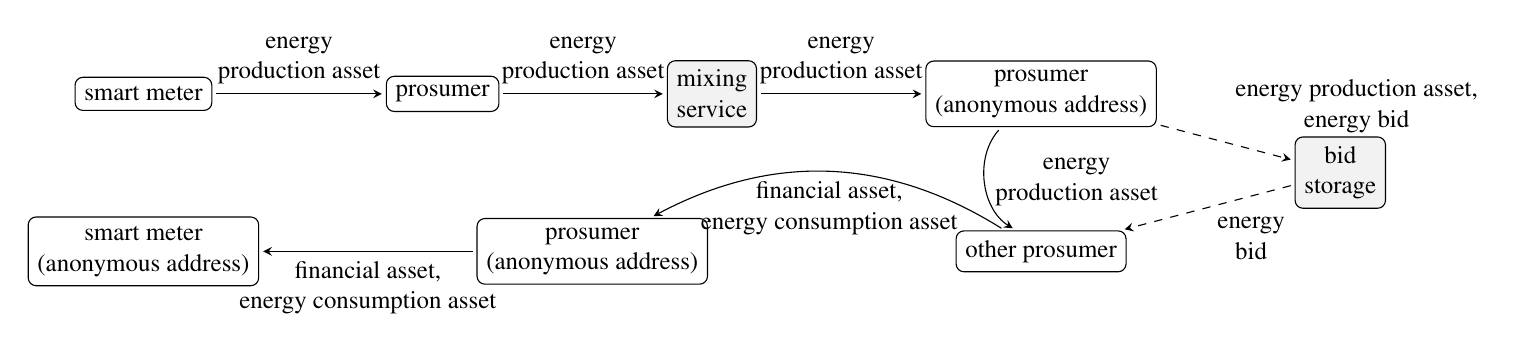
\begin{tikzpicture}[x=3.8cm, y=2cm, font=\small,
  system/.style={draw, align=center, rounded corners=0.1cm, fill=black!5},
  entity/.style={draw, align=center, rounded corners=0.1cm},
  asset/.style={midway, align=center},
  transfer/.style={->, >=stealth, shorten <=0.05cm, shorten >=0.05cm},
]
%\node[entity] (smartmeter) at (0.75, 0.5) {smart\\meter};
%\node[entity] (prosumer1) at (1.25, 1) {prosumer};
%\node[system] (mixing1) at (2, 1) {mixing\\service};
%\node[entity] (prosumer2) at (3, 1) {prosumer\\(alternative address)};
%\node[system] (bidstorage) at (4, 1) {bid\\storage};
%\node[entity] (partner) at (4, 0) {other prosumer};
%\node[entity] (prosumer3) at (3, 0) {prosumer\\(alternative address)};
%\node[system] (mixing2) at (2, 0) {mixing\\service};
%\node[entity] (prosumer4) at (1.25, 0) {prosumer};
\node[entity] (smartmeter) at (0, 1) {smart meter};
\node[entity] (prosumer1) at (1, 1) {prosumer};
\node[system] (mixing1) at (1.9, 1) {mixing\\service};
\node[entity] (prosumer2) at (3, 1) {prosumer\\(anonymous address)};
\node[system] (bidstorage) at (4, 0.5) {bid\\storage};
\node[entity] (partner) at (3, 0) {other prosumer};
\node[entity] (prosumer3) at (1.5, 0) {prosumer\\(anonymous address)};
\node[entity] (smartmeter2) at (0, 0) {smart meter\\(anonymous address)};

%\draw[transfer] (smartmeter) -- node [asset, above left] {energy\\production asset} (prosumer1);
%\draw[transfer] (prosumer1) -- node [asset, above] {energy\\production asset} (mixing1);
%\draw[transfer] (mixing1) -- node [asset, above] {energy\\production asset} (prosumer2);
%\draw[transfer, dashed] (prosumer2) -- node [asset, above] {energy production asset,\\energy bid} (bidstorage);
%\draw[transfer, dashed] (bidstorage) -- node [asset, right] {energy\\bid} (partner);
%\draw[transfer, bend right=15] (partner) to node [asset, below] {financial asset,\\energy\\consumption asset} (prosumer3);
%\draw[transfer, bend right=7.5] (prosumer2) to node [asset, above right] {energy\\prod. asset} (partner);
%\draw[transfer] (prosumer3) -- node [asset, below] {financial asset,\\
%energy consumption asset} (mixing2);
%\draw[transfer] (mixing2) -- node [asset, below] {financial asset,\\energy consumption asset} (prosumer4);
%\draw[transfer] (prosumer4) -- node [asset, below left] {financial\\asset} (smartmeter);

\draw[transfer] (smartmeter) -- node [asset, above] {energy\\production asset} (prosumer1);
\draw[transfer] (prosumer1) -- node [asset, above] {energy\\production asset} (mixing1);
\draw[transfer] (mixing1) -- node [asset, above] {energy\\production asset} (prosumer2);
\draw[transfer, dashed] (prosumer2) -- node [asset, above right] {energy production asset,\\energy bid} (bidstorage);
\draw[transfer, dashed] (bidstorage) -- node [asset, below right] {energy\\bid} (partner);
\draw[transfer, bend right=30] (partner) to node [asset, below] {financial asset,\\energy consumption asset} (prosumer3);
\draw[transfer, bend right=50] (prosumer2) to node [asset, right] {energy\\production asset} (partner);
\draw[transfer] (prosumer3) -- node [asset, below] {financial asset,\\
energy consumption asset} (smartmeter2);
\end{tikzpicture}
\caption{Simplified overview of the flow of assets from the perspective of a prosumer who sells energy. Note that in order to prevent de-anonymization, a prosumer should use multiple addresses and multiple rounds of mixing.}
\label{fig:sellFlow}
\end{figure*}

\subsection{Overview}
We begin with a semi-formal description of the energy trading process from the prosumers' perspective.
In subsequent subsections, we will describe the assets, transactions, and services in our system in more detail.

First, consider a prosumer who would like to sell energy to another prosumer (this case is illustrated in Figure~\ref{fig:sellFlow}).
As its very first step, the prosumer obtains an \emph{energy production asset} from its smart meter.
An energy production asset represents a permission to sell a certain amount of energy, and it is used to enforce safety requirements.
If the prosumer has sufficient unsold production capacity, the smart meter creates and transfers a production asset to the prosumer using a \emph{smart meter transaction}, which is recorded on the distributed ledger.

At this point, the production asset can still be traced back to the prosumer since the ledger is public.
To achieve anonymity, the prosumer transfers the production asset to a \emph{mixing service} using an \emph{energy and financial transaction}, which is also recorded on the distributed ledger.
In turn, the mixing service transfers the production asset to an \emph{anonymous address}\todo{We should probably insert a good definition here for reader who are unfamiliar with blockchain transactions.}, which is randomly generated and controlled by the prosumer.
Since the mixing service transfers assets from multiple prosumers to multiple anonymous addresses at the same time, and the anonymous addresses were chosen at random by the prosumers, the assets cannot be traced back to the original prosumers after mixing.\footnote{Note that prosumers should divide their assets between multiple anonymous addresses; otherwise, each asset might be traced back to its prosumer based on the amount of energy that it contains.}

Now, the prosumer can engage in energy trading anonymously.
To find a trade partner, it can either post an \emph{energy bid} on the bid storage, or simply search the storage for an acceptable \emph{energy ask}.
To post an energy bid, the prosumer first proves to the storage service -- without revealing its original identity -- that it owns a production asset stored at an anonymous address.
It can then post the energy bid, which contains an anonymous communication address\footnote{We discuss communication anonymity later.}, a price, and a reference to the production asset.
If another prosumer, who would like to buy energy, finds the bid acceptable, it can contact the selling prosumer at the communication address given by the bid.



\subsection{Timing}
The ability to specify points or intervals in time is crucial.
For example, control signals specify how the load should change at certain points in time, energy trades specify when energy will be consumed or produced, etc.
To facilitate processing signals and transactions, we divide time into fixed-length intervals, and specify points or periods in time using these discrete timesteps.
The length of the time interval is determined by mapping the timing assumptions of the power system to our platform.
%In our implementation, 
For example, the default length of the time interval may be 4 seconds, which corresponds to how frequently the control signal of the DSO typically changes.

\subsection{Services}

Here, we describe three services that must be implemented for our solution: communication anonymity, mixing service for transaction anonymity, and anonymous bid storage for bidding anonymity.

\subsubsection{Communication Anonymity}
Firstly, we must provide an anonymous communication layer, on which we can build an anonymous trading platform.
Without this communication layer, bids and transactions could be easily de-anonymized based on the network identifiers of the sources (e.g., IP or MAC addresses).

We can employ well-known and widely used techniques for anonymous communication, such as \emph{onion routing}.
To build an onion network, the smart meters, inverters, and other devices can act as onion routers, and the list of onion routers in a microgrid can be published on a private blockchain.
In our first implementation, we can use the free and open-source Tor software with private Directory Authorities.
% ritter.vg: "run your own tor network"
% https://ritter.vg/blog-run_your_own_tor_network.html

\subsubsection{Transaction Anonymity}
We must provide prosumers with the ability to create and publish transactions anonymously.
More specifically, prosumers should be able to purchase or sell energy without revealing their identity; however, these transaction must also be verifiable and enforceable.

We may achieve this goal using multiple approaches for blockchain transaction anonymity:
\begin{itemize}
\item Mixing services (also known as tumblers) mix potentially identifiable assets on a blockchain with others, thereby preventing tracing individual assets back to their original source. 
In our case, assets to be mixed include virtual balances of fiat currencies as well as energy production and consumption.
\item Cryptographic anonymity for transactions is provided, for example, by Zerocoin~\cite{miers2013zerocoin}. Similarly to mixing service, Zerocoin can prevent tracing assets on a blockchain.
\end{itemize}
Using the above techniques, we can enable prosumers to trade energy anonymously (i.e., without revealing their true identities), but at the same time prevent them from altering their energy or financial balances without a valid transaction.

However, we must also ensure that 1) smart meters know the amount of energy purchased or sold by their prosumer and 2) prosumers cannot purchase or sell more energy than their capacity.
To satisfy both of these constraints, all energy trades must start with the prosumer withdrawing a certain amount of energy production or consumption from its smart meter:
\begin{itemize}
\item If a prosumer wishes to sell energy, it must first obtain an energy asset from its smart meter using a blockchain transaction.
This transaction must be signed by the smart meter, which enables the smart meter to 1) keep track of the amount of energy traded by the prosumer as well as to 2) enforce safety requirements by limiting the amount of energy that can be withdrawn.
\item If a prosumer wishes to buy energy, it must first obtain an energy consumption asset from its smart meter in a way similar to obtaining an energy production asset.
\end{itemize}

\subsubsection{Bidding Anonymity}
Finally, we must provide prosumers with the ability to publish energy buy and sell bids anonymously.
To this end, we create a storage for anonymous bids that is readable by all the prosumers in the microgrid.
Any prosumer may submit a bid to this storage; however, in order to do so, they must provide a zero-knowledge proof of owning the assets that are to be traded:
\begin{itemize}
\item To submit an energy sell bid, the prosumer must prove that it owns an energy production asset on the chain.
\item To submit an energy buy bid, the prosumer must prove that it own an energy consumption asset as well as financial assets on the chain.
\end{itemize}


\subsection{Transaction Types}

Before we can discuss transaction types, we must first define the three assets that these transactions may transfer.

An \emph{energy production asset} (EPA) is defined by
\begin{compactitem}
\item \field{power}: non-negative amount of power to produced (for example, measured in watts).
\item \field{start}: first time interval in which energy is to be produced. 
\item \field{end}: last time interval in which energy is to be produced.
\end{compactitem}
An \emph{energy consumption asset} (ECA) is defined by the same fields; however, for this asset, the fields define consumption instead of production.
Finally, a \emph{financial asset} (FA) is defined by a single non-negative field \field{amount}, which can be denominated in either a fiat currency (e.g., US dollars) or a cryptocurrency.

\subsubsection{Energy and Financial Transactions}

Energy and financial transactions transfer energy and financial asset from one address to another.
Prosumers use these transactions for multiple purposes: to trade energy by exchanging assets with other prosumers, to prove to the bid storage that they have production or consumption capacity, to hide their identity by transferring assets to and from mixing services, and to deposit assets at their smart meter.
%
An energy and financial transaction contains the following fields:
\begin{compactitem}
\item List of EPA inputs, each of which is defined by:
\begin{compactitem}
\item \field{out}: EPA output from a previous transaction,
\item \field{sig}: signature for this output.
\end{compactitem}
\item List of ECA inputs, each of which is defined by:
\begin{compactitem}
\item \field{out}: ECA output from a previous transaction,
\item \field{sig}: signature for this output.
\end{compactitem}
\item List of FA inputs, each of which is defined by:
\begin{compactitem}
\item \field{out}: FA output from a previous transaction,
\item \field{sig}: signature for this output.
\end{compactitem}
\item List of EPA outputs, each of which is defined by:
\begin{compactitem}
\item an EPA and an address to which it is transferred.
\end{compactitem}
\item List of ECA outputs, each of which is defined by:
\begin{compactitem}
\item an ECA and an address to which it is transferred.
\end{compactitem}
\item List of FA outputs, each of which is defined by:
\begin{compactitem}
\item an FA and an address to which it is transferred.
\end{compactitem}
\end{compactitem}

An energy and financial transaction is valid if the following three conditions hold.
\begin{compactitem}
\item None of the outputs referenced by the inputs have been spent by a transaction that has been recorded on the ledger.
\item All of the signatures are valid.
\item For each asset type (and for each timestep), the sum of inputs and outputs is the same.
For example, in the case of energy production assets, the condition is:
\begin{align}
\forall t: & \sum_{out \in \text{EPA outputs}} out.\mathtt{power} \cdot 1_{\left\{out.\mathtt{start} \leq t \leq out.\mathtt{end}\right\}} \nonumber \\
& = \sum_{in \in \text{EPA inputs}} in.\mathtt{out}.\mathtt{power} \cdot 1_{\left\{in.\mathtt{out}.\mathtt{start} \leq t \leq in.\mathtt{out}.\mathtt{end}\right\}} ,
\end{align}
where $1_x$ is equal to $1$ if $x$ is true, and it is $0$ otherwise.
%\begin{equation}
%\forall t: \sum_{out \in \left\{out' \middle| out' \in \text{ EPA outputs} \wedge out'.EPA.start \leq t \leq out'.EPA.end\right\}} out.EPA.Power = \sum_{in \in \left\{in' \middle| in' \in \text{ EPA inputs} \wedge in'.EPA.start \leq t \leq in'.EPA.end\right\}} in.EPA.Power .
%\end{equation}
\end{compactitem}
If a transaction submitted to the ledger is valid, it will be permanently recorded.

\subsubsection{Smart-Meter Transactions}

Prosumers use smart-meter transactions to withdraw energy and financial assets from their own smart meters, before they engage in energy trading.
%
A smart-meter transaction contains the following fields:
\begin{compactitem}
\item List of EPA outputs, each of which is defined by:
\begin{compactitem}
\item an EPA and an address to which it is transferred.
\end{compactitem}
\item List of ECA outputs, each of which is defined by:
\begin{compactitem}
\item an ECA and an address to which it is transferred.
\end{compactitem}
\item List of FA outputs, each of which is defined by:
\begin{compactitem}
\item an FA and an address to which it is transferred.
\end{compactitem}
\item \field{id}: Identifier of the smart meter.
\item \field{sig}: Smart meter's signature over the transaction.
\end{compactitem}

A smart-meter transaction is valid if the following two conditions hold:
\begin{compactitem}
\item The smart meter identified in the transaction has been authorized by a regulatory transaction that has been recorded on the ledger.
\item The smart meter's signature is valid.
\end{compactitem}
\todo{To address malfunctioning or compromised smart meters, we could also impose a limit on withdrawals.}

\subsubsection{Regulatory Transactions}

The DSO uses regulatory transactions to authorize or ban smart meters and to control the microgrid load through setting a price policy.
Since these transactions provide a diverse set of functionality, they are divided into two types.

\paragraph{Authorize or Ban Smart Meters}
The DSO uses these transactions to manage the set of authorized smart meters in the microgrid.
Whenever a new smart meter is installed, the DSO notifies the members of the microgrid using a regulatory transaction.
Similarly, whenever a smart meter is deactivated (e.g., because service is stopped or it is believed to be malfunctioning or compromised), the DSO notifies the members of the microgrid using a regulatory transaction.
These transactions contain the following fields:
\begin{compactitem}
\item List of smart meters to be authorized, each of which is defined by:
\begin{compactitem}
\item \field{id}: Identifier of the smart meter.
\item \field{pubkey}: Public key of the smart meter.
\end{compactitem}
\item List of smart meters to be banned, each of which is given using its identifier.
\item \field{time}: Timestep in which smart meters are authorized and banned.
\item \field{sig}: DSO's signature over the transaction.
\end{compactitem}

A regulatory transaction of this type is valid if the following two conditions hold:
\begin{compactitem}
\item The timestep specified in the transaction is in the future.
\item The DSO's signature is valid.
\end{compactitem}

\paragraph{Price Policy}


%!TEX root = paper.tex



\section{Conclusion and Discussion}
\label{sec:discussion}

% This section presents an analysis of PETra and shows that
% it satisfies the security, safety, and privacy requirements formulated
% earlier.

% \subsection{Security}
% Satisfaction of the security requirements follows from:
% \begin{itemize}[noitemsep,topsep=-\parskip]
% \item immutability of transactions in the distributed ledger,
% \item validity of transactions
% \item and tamper-resistance of smart meters.
% \end{itemize}
% Together, these properties ensure that only the right entities may
% create and sign a transaction, that transactions adhere to the rules
% of the trading workflow, and that transactions cannot be tampered
% with. Double-spending is resolved by scanning the blockchain to allow only unique outputs. 

% \subsection{Safety}
% We now demonstrate that faulty or malicious prosumers cannot trade
% excessive amounts of energy if normal prosumers follow the rules of
% the trading workflow.  Due to the rules of the trading workflow, the gross amount of energy sold is less than or equal to the amount of EPA
% obtained by a prosumer.
% %
% A prosumer can obtain EPA either by withdrawing from its smart meter
% or by purchasing from another prosumer.  From its smart meter,
% prosumer can withdraw at most $\field{MAXEPA}$.  Although the
% prosumer may also buy EPA from another prosumer, this constitutes
% buying energy, which decreases the net amount of energy sold with the
% same amount.  Hence, the net amount of energy sold by prosumer
% cannot exceed $\field{MAXEPA}$.  By extending the argument, we can
% show that the net amount of energy sold by a group of prosumers~$G$
% cannot exceed $\sum_{i \in G} \field{MAXEPA}_i$.  Similarly, %we can
% %show that
%  the net amount of energy bought by a group of prosumers $G$
% cannot exceed $\sum_{i \in G} \field{MAXECA}_i$.

%Using a similar argument, we can also show that the total amount of energy bids (or asks) posted at
%the same time by prosumer $i$ for each timestep is at most
%$\field{MAXEPA}_i + \field{MAXECA}_i$.  This limit is higher than for
%net energy sold or bought, since prosumer $i$ may purchase
%$\field{MAXECA}_i$ amount of EPA (or $\field{MAXEPA}_i$ amount of ECA)
%from other prosumers, and then post an energy ask (or bid) in the
%amount of $\field{MAXEPA}_i + \field{MAXECA}_i$.

Through the use of garlic routing and ring signatures, complete communication and transaction anonymity is achieved. A garlic routing network such as I2P can ensure that no usage, bid, ask or identifiable data is leaked from the system. By using ring signatures, transactions cannot be traced, but it can still be proven that a bid or an ask has been responded to and that a transaction has taken place. The design we've proposed anonymizes the whole chain of transactions, both on a network communication layer and on a distributed ledger transaction layer.

As for the DSO, it receives the same information from the smart meter
as in a non-transactive smart grid (i.e., amount of energy
produced and consumed). In
particular, since price policies are recorded on the ledger (which the
smart meters may read), each prosumer's smart meter may calculate and
send the prosumer's monthly bill to the DSO, without revealing the
prosumer's energy consumption or production. The DSO still gets aggregate information regarding load on the grid, but cannot identify individual users and their energy prosumption. 





%!TEX root = paper.tex
\section{Related Work}
\label{sec:related}

%In this section we describe the related research. It has been divided into two subsections to focus on blockchains, which we are using to implement the distributed ledger service described earlier, and other works on smart grid privacy concerns. 

%\subsection{Smart Grid and Meter Privacy}
% http://ieeexplore.ieee.org/abstract/document/5054916/
%McDaniel and McLaughlin discuss privacy challenges in smart grids~\cite{mcdaniel2009security}.
% https://arxiv.org/pdf/1108.2234.pdf
% https://pdfs.semanticscholar.org/cdf8/a5b6256823bca38a1d2347ab36f8e4a2ca94.pdf
% http://www.comm.toronto.edu/~akhisti/sm.pdf
% https://www.researchgate.net/profile/Georgios_Kalogridis/publication/224189766_Smart_Grid_Privacy_via_Anonymization_of_Smart_Metering_Data/links/541169510cf2b4da1bec4193.pdf
% https://arxiv.org/pdf/1305.0735.pdf
New privacy concerns arise with the continuing adoption of smart
grids. In addition to old and new security threats (such as energy
theft and smart-meter malware), McDaniel and McLaughlin discuss the
privacy concerns of energy usage profiling that smart grids could
potentially enable~\cite{mcdaniel2009security}. Several approaches
have been investigated as potential means to provide privacy
protections for smart grid users.

Some approaches look to the use of protocols and/or frameworks to help
protect privacy. Rajagopalan et al.\ use tools from information theory
to present a framework that abstracts both the privacy and the utility
requirements of smart-meter
data~\cite{rajagopalan2011smart,sankar2013smart}. Their framework
leads to a novel tractable privacy-utility tradeoff problem with
minimal assumptions. Efthymiou and Kalogridis describe a method for
securely anonymizing frequent electrical metering data sent by a smart
meter~\cite{efthymiou2010smart}. Their approach is based on the
observation that frequent metering data may be required by an energy
distribution network for operational reasons, but it may not
necessarily need to be attributable to a specific smart meter. The
authors describe a method that provides a third-party escrow mechanism
for authenticated anonymous meter readings, which are hard to
associate with a particular smart meter.

Other approaches, such as additional hardware components, have also been explored 
for potential privacy gains. 
Varodayan and Khisti study using a
rechargeable battery for partially protecting the privacy of
information contained in a household's electrical load
profile~\cite{varodayan2011smart}. They show that stochastic battery
policies may leak 26\% less information than a best-effort policy,
which holds the output load constant whenever possible. Tan et
al.\ study privacy in a smart metering system from an information
theoretic perspective in the presence of energy harvesting and storage
units~\cite{tan2013increasing}. They show that energy harvesting
provides increased privacy by diversifying the energy source, while a
storage device can be used to increase both energy efficiency and
privacy.
% They show that there exists a trade-off between the information
% leakage rate and the wasted energy rate, and study the impact of the
% energy harvesting rate and the size of the storage device on this trade-off.

PETra extends this work by (1) leveraging a decentralized IoT
system for transactive energy and (2) addressing the novel privacy
threat posed by trading. In particular, while earlier work protected
the prosumers' privacy from the DSO, PETra also protects it from other
prosumers, as well as outside attackers.

A key element of PETra is its ability to distribute information among
peers via blockchains.  As blockchain technology develops and matures,
new frameworks, services, and protocols are being developed to
leverage the distributed ledgers provided by blockchains. For example,
Hyperledger Fabric is a platform for distributed ledger solutions,
which was designed to support pluggable implementations of different
components~\cite{hyperledger2017fabric}.
%Bitcoin Lightning Network is
%decentralized system, in which transactions are sent over a network of
%micropayment channels, whose transfer of value occurs
%off-blockchain~\cite{poon2016bitcoin}. 
Since this paper focuses on the theoretical foundations of PETra, any
of these distributed ledgers provide the required capabilities.

%\Abhishek{Aron this section should end with a few sentence about how our approach fits in. Perhaps just a few sentences reworded from introduction will be sufficient}

\iffalse
\subsection{Blockchains as Distributed Ledgers}

As Blockchain technology continues to develop and mature, new
frameworks, services, and protocols are being developed to leverage
blockchain's distributed ledger. Microsoft offers Blockchain as a
Service (BaaS) on Azure. Additionally, Microsoft has Project Bletchley
as its architectural approach to building an Enterprise Consortium
Blockchain Ecosystem, introducing two new concepts: blockchain
middleware and a secure means for calling code or data outside a
SmartContract or blockchain called
cryptlets~\cite{gray2016introducing}. Hyperledger Fabric is a platform
for distributed ledger solutions, which was designed to support
pluggable implementations of different
components~\cite{hyperledger2017fabric}. Bitcoin Lightning Network is
decentralized system, in which transactions are sent over a network of
micropayment channels whose transfer of value occurs
off-blockchain~\cite{poon2016bitcoin}. Interledger is a protocol for
payments across payment systems, which enables anyone with accounts on
two ledgers to create a connection between
them~\cite{thomas_protocol}. Xu et al.\ discuss the use of two pools
of proxy agents, an agreement pool and a payment pool, to assist in
protection of privacy when using blockchain technologies for
transactions on tangible goods~\cite{Xu2017}.  \fi

%\url{https://geli.net/residential/}
%\url{https://www.greentechmedia.com/articles/read/geli-raises-7m-to-take-energy-storage-software-to-the-next-level}

%\url{http://ethembedded.com/}


\section{Conclusion}
\label{sec:conclusion}

In this paper, we described the design and implementation of a  transaction management platform (TMP) for IoT-based transactive microgrids. Our solution enables prosumers to trade energy without threatening their privacy or the safety of the system. Our hybrid solver approach, which combines a smart-contract based validator with an external optimizer, enables the platform to clear offers securely and efficiently. Further, the ability to trade across multiple time intervals enables participants to take full advantage of batteries, thereby smoothening the load on the main grid. Finally, the use of blockchains provides decentralized trust and consensus capabilities, which protect from  malicious actors.


\AronC{future work:
- recovery from failures: retroactively change matching in case of a physical failure

- fault-tolerant matching: safety constraints will be satisfied even if a certain number of physical elements fail (or prosumers get disconnected)

- propose alternative market mechanisms, including those that involve double auctions and its variants.}




% BALANCE COLUMNS
%\balance{}
%\setlength{\bibsep}{0pt plus 0ex}
\let\oldthebibliography\thebibliography
\let\endoldthebibliography\endthebibliography
\renewenvironment{thebibliography}[1]{
  \begin{oldthebibliography}{#1}
    \setlength{\itemsep}{0.1em}
    \setlength{\parskip}{0em}
}
{
  \end{oldthebibliography}
}

\vspace{-0.1in}
% REFERENCES FORMAT
% References must be the same font size as other body text.
\bibliographystyle{SIGCHI-Reference-Format}

\bibliography{references}

\end{document}

